% reducesymm/QFT/QFTBlog.tex
% Predrag  switched to github.com               jul  8 2013

\chapter{Daily QFT blog}
\label{c-DailyBlog}

\begin{description}
%\item[2013-11-23  Predrag] Moved all matters QFT from
%\texttt{siminos/blog/Lie.txt} to here.

\item[2010-03-04 Predrag]
Kevin Mitchell is here, says we should study Littlejohn and
M. Reinsch\rf{LiRe97}: ``Gauge fields in the separation of
rotations and internal motions in the $n$-body problem.'' I
will put it into \wwwcb{/library}. Read 3-body problem
sections. See p. 14 for a discussion of the three-body
coordinates and p. 25 for a discussion of the three-body
section (gauge).



\item[2011-07-27 PC]
What follows is casting eye far ahead - to the role of gauge invariance
in Quantum Field Theories.
Following articles seem of interest as follow-ups on
Cvitanovi\'c\rf{PCar}, {\em Group theory for {Feynman} diagrams in
non-{Abelian} gauge theories}:

Khellat\rf{Khel10} strikes me as dubious...

Martens\rf{Mart11} writes: ``We calculate the two-loop matching corrections for the
   gauge couplings at the Grand Unification scale in a general framework
   that aims at making as few assumptions on the underlying Grand Unified
   Theory (GUT) as possible. In this paper we present an intermediate
   result that is general enough to be applied to the Georgi-Glashow
   SU(5) as a ``toy model''. The numerical effects in this theory are
   found to be larger than the current experimental uncertainty on $\alpha$s .
   Furthermore, we give many technical details regarding renormalization
   procedure, tadpole terms, gauge fixing and the treatment of group
   theory factors, which is useful preparative work for the extension of
   the calculation to supersymmetric GUTs.
   ''

Tye and Zhang\rf{TyZh10} write: ``
Bern, Carrasco and Johansson have conjectured dual
   identities inside the gluon tree scattering amplitudes.
   We use the properties of the heterotic string and open string tree
   scattering amplitudes to refine and derive these dual identities.
   These identities can be carried over to loop amplitudes using the
   unitarity method. Furthermore, given the $M$-gluon (as well as
   gluon-gluino) tree amplitudes, $M$-graviton (as well as
   graviton-gravitino) tree scattering amplitudes can be written down
   immediately, avoiding the derivation of Feynman rules and the
   evaluation of Feynman diagrams for graviton scattering amplitudes

Eto \etal\rf{EFGKNOV08} write:
   ``We construct the general vortex solution in the color-flavor-locked
   vacuum of a non-Abelian gauge theory, where the gauge group is taken
   to be the product of an arbitrary simple group and U(1). Use of the
   holomorphic invariants allows us to extend the moduli-matrix method
   and to determine the vortex moduli space in all cases. Our approach
   provides a new framework for studying solitons of non-Abelian
   varieties with various possible applications in physics.''

and there is much much more...; will continue some other time.

\item[2011-11-03 PC] Today is that time. I'm sitting in
\HREF{http://intractability.princeton.edu/blog/2011/05/workshop-counting-inference-and-optimization-on-graphs/}
     {Intractability Workshop:}
     \emph{Counting, Inference and Optimization on Graphs}
with a bunch of high-level computer nerds, and I almost afraid to say
what I'll say next (plumbers avoid physicists that say such things): In
constructing our atlas of inertial manifold of turbulent pipe flow, we
fix the $SO(2) \times O(2)$ phase separately on each local chart. The
freedom of doing that is called ``local gauge invariance'' (blame Hermann
Weyl for the ugly word) and in the limit of $\infty$ period cycles, cycle
points are dense and their local charts are infinitesimal, so this is
really local gauge invariance. In the world of computer science they use
this freedom profitably, to reduce the number of terms they use in their
computations. That suggests that there might be a (variational?)
principle that selects an optimal choice of (relative) template phases
(\ie, gauge transformations that connect a chart to the next chart).

Nerds call this 'reparametrization' - it supposedly speeds up calculations.
Have not really seen that in quantum field theory, with exception of light
cone gauges and their relatively recent applications by the Witten cult.

Literature: \refref{CheChe08,YeChe11} and stuff on
\HREF{http://www.hpl.hp.com/personal/Pascal_Vontobel/ciog2011/reading_list_web.html}{this
site} (if you can understand any of it).

Feel free to ignore this remark. It's future research.

\item[2012-05-16  Parameswaran Nair]  vpnair@optonline.net writes
on saddle solutions of Yang-Mills:

I attributed the conjecture to Hitchin; it was actually due to Atiyah and
Jones. ''The only finite action solutions of the YM equations are
instantons, either self-dual or antiself-dual.'' This was the conjecture
for which the refs provide counter examples.

\HREF{http://ChaosBook.org/library/Schiff91.pdf}{Here is} the paper by my
student Schiff\rf{Schiff91}, who writes:
``
Following a proposal of Burzlaff (Phys.Rev.D 24 (1981) 546), we find
solutions of the classical equations of motion of an abelian Higgs model
on hyperbolic space, and thereby obtain a series of non-self-dual
classical solutions of four-dimensional SU(3) gauge theory. The lowest
value of the action for these solutions is roughly 3.3 times the standard
instanton action.
''

``
In physics, despite the fact that the non-self-dual solutions correspond
to saddle points, and not minima, of the Yang-Mills functional, to do a
correct semiclassical approximation by a saddle-point evaluation of the
path integral, it is certainly necessary to include a contribution due to
nonself-dual solutions, and if it should be the case that there is a
non-self-dual solution with action lower than the instanton action (this
question is currently open, and of substantial importance), then such a
contribution would even dominate. Unfortunately, it is questionable
whether the semiclassical approximation can give a reliable picture of
quantized gauge theories; it has been argued that in four-dimensional
gauge theory small quantum fluctuations
around classical solutions cannot be responsible for
confinement, unlike in certain lower-dimensional
theories. But it may still be possible to extract some
physics from the semiclassical approach. A first step in
such a direction would be to obtain a good understanding
of the full set of non-self-dual solutions and their properties.
[...] We pursue an old idea, due to Burzlaft
[10], for obtaining a non-self-dual, ''cylindrically symmetric''
solution for gauge group SU(3). If we write
$\reals^4 = \reals \times \reals^3$, and identify some SU(2) [or SO(3)] subgroup
of SU(3), with generators that we will denote T', then we
can look at the set of SU(3) gauge potentials which are invariant
under the action of the group generated by the
sum of the T''s and the generators of rotations on the IR
factor of E (we choose the T''s and the IR rotation generators
to satisfy the same commutation relations). We
call such potentials ''cylindrically symmetric'' (in analogy
to the standard notion of cylindrical symmetry in IR,
which involves writing R =RXIR and requiring rotational
symmetry on the E factor). Such potentials will
be specified by a number of functions of two variables:
the coordinate on the IR factor of E (which we will
denote x), and the radial coordinate of the E factor
(which we will denote y). Clearly the equations of motion
for such cylindrically symmetric potentials (if they are
consistent) will reduce to equations on the space
I (x,y ):y ~ 0].
,,

The earlier work is by Sibner, Sibner, Uhlenbeck\rf{SiSiUhl89}. They
write ``
The Yang-Mills functional for connections on principle SU(2) bundles over
S 4 is studied. Critical points of the functional satisfy a system of
second-order partial differential equations, the Yang-Mills equations. If,
in particular, the critical point is a minimum, it satisfies a
first-order system, the self-dual or anti-self-dual equations. Here, we
exhibit an infinite number of finite-action non-minimal unstable critical
points. They are obtained by constructing a topologically nontrivial loop
of connections to which min-max theory is applied. The construction
exploits the fundamental relationship between certain invariant
instantons on S 4 and magnetic monopoles on H 3. This result settles a
question in gauge field theory that has been open for many years.
''

% 2012-05-16 fund this:
%@article{
%author = {Gil Bor and Richard Montgomery},
%title = {{SO(3)} invariant {Yang-Mills} fields which are not self-dual},
%}

Bor\rf{Bor92} writes
``
We prove the existence of a new family of non-self-dual finite-energy
solutions to the Yang-Mills equations on Euclidean four-space, with SU(2)
as a gauge group. The approach is that of ``equivariant geometry:''
attention is restricted to a special class of fields, those that satisfy
a certain kind of rotational symmetry, for which it is proved that (1) a
solution to the Yang-Mills equations exists among them; and (2) no
solution to the self-duality equations exists among them. The first
assertion is proved by an application of the direct method of the
calculus of variations (existence and regularity of minimizers), and the
second assertion by studying the symmetry properties of the linearized
self-duality equations. The same technique yields a new family of
non-self-dual solutions on the complex projective plane.
''

\item[2012-04-19 Daniel] ``graveyard of obvious ideas'' rings a little
    aggressive, no? ``if you are a master of quantum-mechanics or QFT symmetries
and their linear irreducible representations,\rf{PCgr} you may leave your
baggage at the door'' rings a little aggressive, too.
\\{\bf Predrag:} Get's edgy. In ``master of their linear irreducible
    representations'' I make fun of myself. Let the referee object to
    that?


{\bf [2012-06-14 Predrag]} Grin and bear it. Pulling my Senior discount
card here.

\item[2013-07-15, 2018-08-27 Predrag]
I've collected a bunch of QFT e-books, saved
them in \wwwcb{/library}:

Grigorenko 2006 \CBlibrary{5449Grigorenko06}

Abarbanel 2013 \CBlibrary{Abarbanel 2013}

Altland and Simons\rf{AltlSim09}
{\em Condensed Matter Field Theory}:
see Chapter~1 {\em Collective Excitations: From
Particles to Fields} \CBlibrary{AltlSim-Chap1}.

Check out also

\HREF{https://www.tcm.phy.cam.ac.uk/~bds10} {Simons},
Lecture I:
\HREF{https://www.tcm.phy.cam.ac.uk/~bds10/tp3/lectures.pdf}
{\em Collective Excitations:  From Particles to Fields
Free Scalar Field Theory:  Phonons}

Simons
\HREF{http://www.tcm.phy.cam.ac.uk/~bds10/tp3.html}
{\em Quantum Condensed Matter Field Theory}

T. Banks\rf{Banks08},
{\em Modern Quantum Field Theory: A Concise Introduction}
download from
\HREF{http://web.phys.ntnu.no/~mika/banks.pdf} {here},
review \HREF{https://doi.org/10.1080/00107510903073286} {here} :\\
\CBlibrary{Banks08}

Chaichian and A. Demichev\rf{Chaichian01Vol1}
{\em Path Integrals in Physics
Volume I
Stochastic Processes and Quantum Mechanics}:
\CBlibrary{Chaichian01Vol1}

Chaichian and A. Demichev\rf{Chaichian01Vol2}
{\em Path Integrals in Physics
Volume  II
Quantum Field Theory, Statistical Physics and other Modern Applications}:
\CBlibrary{Chaichian01Vol2}

\HREF{http://www.physics.rutgers.edu/~coleman/}
{Piers Coleman}\rf{Coleman15} {\em Introduction to Many-Body Physics}:
\CBlibrary{Coleman15a} + \CBlibrary{Coleman15b}

CoKaWa 2004 \CBlibrary{CoKaWa04}

DasFerbel 2003 \CBlibrary{DasFerbel03}

Farmelo\rf{DiracLife}
{\em The Strangest Man: The Hidden Life of Paul Dirac, Mystic of the Atom}:
\CBlibrary{DiracLife}

Hao 1989 \CBlibrary{hao89}

Nichkawde 2013 \CBlibrary{Nichkawde13}

Das 2006 \CBlibrary{Das06}

Elvang and Huang\rf{ElHu13,ElHu15} {\em Scattering Amplitudes}, \arXiv{1308.1697}

Milton 2001 \CBlibrary{Milton01}

NagashimaI 2010 \CBlibrary{NagashimaI10}

Elbaz\rf{Elbaz12}: \CBlibrary{Elbaz12}

Sadovskii\rf{Sadovskii13} {\em Quantum Field Theory}:
\CBlibrary{Sadovskii13}

Sadovskii\rf{Sadovskii06}
{\em Diagrammatics: Lectures on Selected Problems in Condensed Matter Theory}
\CBlibrary{Sadovskii06}

SeoSan 2012 \CBlibrary{SeoSan12}

Szekeres\rf{Szekeres04} {\em A Course in Modern Mathematical Physics: Groups,
Hilbert Space and Differential Geometry}:
\HREF{http://ChaosBook.org/library/Szekeres04.djvu} { (click here)}

Zee 2003 \CBlibrary{Zee03}

\HREF{http://web.mit.edu/redingtn/www/netadv/biblio2.html\#strintsys}
{An online references list}

Howard Haber \HREF{http://scipp.ucsc.edu/~haber/ph218/} {list of sources}

\item[2013-04-16  Predrag] There seems to be whole literature on
classical Yang-Mills (CYM). In
{\em Entropy production in classical Yang-Mills theory from Glasma
initial conditions} Hideaki Iida,  Teiji Kunihiro,  Berndt M\"uller,
Akira Ohnishi,  Andreas Sch\"afer,  and Toru T. Takahashi,
\arXiv{1304.1807}, % \rf{IKMOST13}
write:

Pure Yang-Mills theory in temporal gauge with the Hamiltonian in the
noncompact (A, E) scheme on a cubic spatial lattice. The initial
condition satisfies Gauss' law; check its validity as well as Energy
conservation carefully at every time step. Define distance (6), (7) that
is gauge invariant under residual (time independent) gauge transformations.

                                                    \inCB
They call the stability matrix `Hessian', and its eigenvalues at time
slice the `local Lyapunov exponents (LLEs)'\rf{KMOSTY10}: LLE plays the
role of a ``temporally local'' Lyapunov exponent, which specifies the
departure rate of two trajectories in a short time period. Then they say
this (?): ``For a system where stable and unstable modes couple with each
other as in the present case, an LLE does not generally agree with the
Lyapunov exponent in a long time period.'' ``\refRef{KMOSTY10} introduced
another kind of Lyapunov exponent called the intermediate Lyapunov
exponent (ILE), which is an ``averaged Lyapunov exponent'' for an
intermediate time period; i.e., a time period which is sufficiently small
compared to the thermalization time but large enough to sample a
significant fraction of phase space. By its definition (13) it
is the set of stability exponents for a finite time \jacobianM.

``Two comments are in order, here: A Lyapunov exponent [PC: not the
Lyapunov exponent, they mean the stability exponent] can be (real)
positive, negative, zero or purely imaginary. Liouville's theorem tells
us that the determinant of the time evolution matrix U is unity, implying
that the sum of all positive and negative ILEs is zero. The KS entropy is
given as a sum of positive Lyapunov exponents. The second comment
concerns gauge invariance of the Lyapunov exponents. In the Appendix we
show that LLE and ILE are indeed gauge invariant under time-independent
gauge transformations in the temporal gauge.''

\item[2013-11-27  Predrag] One way to reduce symmetry seems obvious;
\textbf{average over the group orbit}. That reduces the dimension of the \statesp\
by the dimension of the group orbit; in the reduced \statesp\ each group
orbit is replaced by a point, it's average value. It is a natural construct
in the theory of linear
representations of groups, very important, where it is called a
`character' of the representation; I use it in my
\HREF{http://chaosbook.org/~predrag/papers/Cvi07.pdf} {trace formula} for
systems with continuous symmetries. But it is a trace of a linear evolution
operator.

Still, I do not seem to know how to do this for (1) nonlinear systems,
(2) QFT gauge fixing. Barth and Christensen\rf{BarChr83}  is an example
where this is done - perhaps a way too complicated example... (here are
my notes \HREF{http://chaosbook.org/FieldTheory/extras/BarChr83note.pdf}
{on it}, which I no longer understand myself :)

\item[2014-01-11 Predrag]
I always wonder whether we should be reducing symmetries
by averaging over group orbits (method of characters, used in
my derivation of the {\Fd} in presence of continuous symmetries).
Churchill, Kummer and Rod\rf{ChKuRo83} write in
{\em On averaging, reduction, and symmetry in {Hamiltonian} systems}:
The existence of periodic orbits for Hamiltonian systems at
low positive energies can be deduced from the existence of nondegenerate
critical points of an averaged Hamiltonian on an associated ``reduced
space.'' The paper exploits discrete symmetries, including reversing
diffeomorphisms, that occur in a given system. The symmetries are used to
locate the periodic orbits in the averaged Hamiltonian, and thence in the
original Hamiltonian when the periodic orbits are continued under
perturbations admitting the same symmetries.''

\item[2014-01-11 Predrag]
Kummer\rf{Kummer81}, {\em On the construction of the reduced phase space
of a {Hamiltonian} system with symmetry} writes:
``
Weinstein [...] uses this correspondence between connections
and lifts in his construction of Sternberg's phase space for a
particle in a Yang-Mills field.
''

l. A. Weinstein, A universal phase space for particles in Yang-Mills
fields, Lett. Math. Phys. 2 (1978), 417-420. \\
2. S. STERNBERG, Minimal coupling and the symplectic mechanics of a
classical particle in the presence of a Yang-Mills field, Proc. Nat.
Acad. Sci. 74 (1977),5253-5254. \\
3. S. STERNBERG, On the role of field theories in our physical conception
of geometry in Differential geometric methods in mathematical physics II,
Springer Lecture Notes in Mathematics,
676 (1977), 1-80. \\

\item[2014-07-30 Predrag]
Paul Hoyer recent talk at
\HREF{http://www.physics.ncsu.edu/LC2014/LC2014-Friday/PaulHoyer.pdf}
{Light Cone 2014} is too packed to be useful, but maybe has some pointers
to recent interesting non-perturbative QCD results.

\item[2014-08-01 Burak]
Sydney Coleman\rf{Col77} gave a lecture on semi-classical formulations of QFT in 1975.
He has several semi-classical treatment methods with names
``Zeroth-Order Weak-Coupling Expansion",
``Coherent-State Variation",
``First-Order Weak-Coupling Expansion",
``Bohr-Sommerfeld Quantization", and
``DHN Formula". I didn't yet understand what any of these means, I'm just starting
to read it, but if we can find a way of adapting these methods to the numerical
calculations that might be a good starting point.

\item[2014-08-01 Predrag]
Coleman was a great expositor - on a level of a Nobelist. Would be cute
if we found something in his lectures we can use today. ``DHN Formula" (I
knew all three - the first two authors are currently dead) should be the
Gutzwiller formula for QFT. Paolo Muratore-Ginanneschi, a former student
in our Copenhagen group, wrote something on that\rf{Murat03} that I still
have not studied in depth. But we maybe should.

\item[2014-08-01 Burak]
Coleman refers to the pedagogical overview by Rajaraman\rf{Raj75} for the derivation
of ``DHN Formula'' and I think this will be a good starting point for me. So far,
keywords are familiar, in the introduction, he talks about periodic orbits and
their stability and how hard it is to find them for realistic cases. A lot of work
apparently in this period has been done using Sine-Gordon equation because they
had analytical solutions. I looked for articles which cite \rf{Raj75} but didn't
see anything that relies on numerical solutions of field equations.

\item[2014-08-13 Predrag]
In my notes it says that Dyson himself told me to read {\em Drawing
theories apart: the dispersion of {Feynman} diagrams in postwar physics},
by Kaiser\rf{Kaiser09}. So we better read it - I will put a pilfered
eBook copy \HREF{http://ChaosBook.org/library/Kaiser09.pdf}{Kaiser09.pdf}
into ChaosBook.org/library.

\item[2014-11-05 Predrag]
Do not know if this is something for us, but worth having a look at:

Luca Salasnich,
 \emph{Discrete bright solitons in Bose-Einstein condensates and dimensional
  reduction in quantum field theory}, \arXiv{1411.0160}:
`` We  review the derivation of an effective one-dimensional (1D) discrete
nonpolynomial Schr\"odinger equation from the continuous 3D Gross-Pitaevskii
equation with transverse harmonic confinement and axial periodic potential.
Then we study the bright solitons obtained from this discrete nonpolynomial
equation showing that they give rise to the collapse of the condensate above a
critical attractive strength. We also investigate the dimensional reduction of
a bosonic quantum field theory, deriving an effective 1D nonpolynomial
Heisenberg equation from the 3D Heisenberg equation of the continuous bosonic
field operator under the action of transverse harmonic confinement. Moreover,
by taking into account the presence of an axial periodic potential we find a
generalized Bose-Hubbard model which reduces to the familiar 1D Bose-Hubbard
Hamiltonian only if a strong inequality is satisfied. Remarkably, in the
absence of axial periodic potential our 1D nonpolynomial Heisenberg equation
gives the generalized Lieb-Liniger theory we obtained some years ago.''

\item[2014-11-23 Predrag]
Zvonkin\rf{Zvonkin97} \CBlibrary{Zvonkin97}
writes in
{\em Matrix integrals and map enumeration: {An} accessible introduction}:
``Physicists working in two-dimensional quantum gravity invented a new
method of map enumeration based on computation of Gaussian integrals over
the space of Hermitian matrices. This paper explains the basic facts of
the method and provides an accessible introduction to the subject.''

\item[2015-01-09 Predrag]

Tudor Dimofte gave a talk in Math on
{\em Geometric representation theory, symplectic duality, and 3d
supersymmetric gauge theory}

Abstract: Recently, a ``symplectic duality" between D-modules on certain
pairs of algebraic symplectic manifolds was discovered, generalizing
classic work of Beilinson-Ginzburg-Soergel in geometric representation
theory. I will discuss how such dual spaces (some known and some new) arise
naturally in supersymmetric gauge theory in three dimensions.

Tudor is a mathematical physicist at the IAS,
School of Physics, Princeton.

I went to the talk, and - wow! You would think I know something about a
gauge theory but is is like it was in Lithuanian: I understood individual
words, and the alphabet seemed to be Latin - there were things that
looked like letter G or letter H and what we call quotient M/G is
apparently called `resolution'. The foundational paper is Braden, Licata,
Proudfoot and Webster\rf{BrLiPrWe12}, and its followups on
``Quantizations of conical symplectic resolutions II: category O and
symplectic duality''. Good luck reading these...

and of course, it was emphatically N=4 and not N=2, so now I'm at peace

:)

\item[2015-02-04 Predrag] Stephan Stetina
    <stetina@hep.itp.tuwien.ac.at> thesis \\
    on \arXiv{1502.00122} uses my
    \HREF{http://chaosbook.org/fieldtheory/} {Field Theory}, and says
    that 2PI graphs are no sweat (for me they were). Wrote to him:

You seem to have
\HREF{http://chaosbook.blogspot.com/1985/05/feynmans-review-of-my-field-theory-book.html}
{proven Feynman wrong} :) That's no mean achievement. Congrats!

Me and my friends have been studying turbulence in fluid dynamics as a
warmup for doing the same in Yang-Mills. If you see some interesting
turbulence in relativistic fluid dynamics, we are always willing to have
a look at things more field-theoretical.

\item[2015-02-09 Stephan Stetina]
If you are referring to Feynman comments on your book, I definitely disagree
with them - I found your book on field theory more than helpful!

It is very difficult to study (quantum) turbulence within our approach -
however it would be very interesting to do so! The original idea was to
derive the two-fluid hydrodynamics of superfluids from an underlying
field theory. To be able to obtain analytical results, we had to apply
some rather drastic simplifications:

We assumed the superfluid condensate to be uniform and homogeneous (which
translate in a homogeneous superflow in the hydro picture). Further more
we used imaginary time formalism which strictly limits us to study
systems in equilibrium. It would most likely be very challenging (in
particular numerically) to introduce a condensate with arbitrary space
and time dependence. In the current calculations, a probable onset of
turbulence manifests itself as "something going wrong" - for example
above certain velocities of the superfluid it is no longer possible to
construct a stable and homogeneous superfluid phase. Another example is
the appearance of the ``two-stream instability" which can also be detected
in our approach (see for instance \arXiv{1312.5993}).
I am not sure yet how much this approach has in common with the one you
have cited.

\item[2015-08-20 Predrag]
Strauss, Horwitz, Levitan, and Yahalom\rf{SHLY15}
{\em Quantum field theory of classically unstable {Hamiltonian} dynamics}
might be a good starting point to learn about dynamical systems for which
the motions can be described in terms of geodesics on a manifold. They
say : ``
... ordinary potential models can be cast into this form by means of a
conformal map. The geodesic deviation equation of Jacobi, constructed
with a second covariant derivative, is unitarily equivalent to that of a
parametric harmonic oscillator, and we study the second quantization of
this oscillator. The excitations of the Fock space modes correspond to
the emission and absorption of quanta into the dynamical medium, thus
associating unstable behavior of the dynamical system with calculable
fluctuations in an ensemble with possible thermodynamic consequences.
''

\item[2016-01-08 Predrag]
Bogomolny wants us to study Englert and
Schwinger\rf{EnglSchw85a,EnglSchw85b,EnglSchw85c}. Why?
\refRef{EnglSchw85a} {\em Semiclassical atom} seems to be reinventing
Gutzwiller, without citing him. These papers are not cited much either, a
pair of Nobel prizes notwithstanding :) Rohwedder and
Englert\rf{RohEng94} continue with {\em Semiclassical quantization in
momentum space}. There is something called the Englert-Schwinger equation
used in graphite studies\rf{ManSan86}. Ullmo~\etal\rf{UNTB01} cite it:
{\em Semiclassical density functional theory: {Strutinsky} energy
corrections in quantum dots}

\item[2016-04-06 Predrag]
Went to hear
\HREF{https://math.berkeley.edu/people/faculty/sung-jin-oh}
{Sung-Jin Oh} talk about

\begin{quote}
``... wave equations that arise from geometric
considerations. Prime examples include the wave map equation and
the Yang-Mills equation on the Minkowski space. On one hand, these
are fundamental field theories arising in physics; on the other hand,
they may be thought of as the hyperbolic analogues of the harmonic map
and the elliptic Yang-Mills equations, which are interesting geometric
PDEs on their own. I will discuss the recent progress on the problem of
global regularity and asymptotic behavior of solutions to these PDEs.''
\end{quote}

This kind of work might offer a path to computing non-trivial ``exact
coherent states'' (non-perturbative classical solutions) of Yang-Mills.
Experimentally I used Evernote on my phone to take notes and photos of
the white board -
\HREF{160406SungJinOh.pdf} {160406SungJinOh.pdf} in this repository -
maybe it helps if one wants to get started reading the literature, though
it is going to be hard going.

Both in the Abelian case (what they call ``Maxwell-Klein-Gordon'' for a
scalar charged particle and ``Maxwell-Dirac'' for spin 1/2), and in the
non-Abelian case (what they call ``Yang-Mills'') they cheerfully set the
particle mass to $m=0$, which is a killer for us.

I tried to briefly explain to Sung-Jin Oh two things of possible interest
to people solving the classical Maxwell-Klein-Gordon and Yang-Mills PDEs:

\begin{enumerate}
  \item
\HREF{http://chaosbook.org/~predrag/papers/preprints.html\#FiniteFieldTheo}
{finiteness conjecture}: perhaps they can find saddle-points
(non-perturbative classical solutions of QED) that give the
gauge sets as the starting step in perturbative calculations,
rather than computing Feynman-diagrammatic corrections to trivial vacuum.

My explanation probably did more harm than good, as I liberally mixed in
QFT, and kept confusing the quantum and the classical problem - it is for
a reason that PDE people do not know what expressions like
``on-mass-shell amplitudes" and ``Ward identities" mean.

  \item
I ran Sung-Jin Oh quickly through \HREF{http://chaosbook.org/tutorials/}
{ChaosBook.org/tutorials} to make him aware that for turbulent nonlinear
PDEs one has to work in the $\infty$\dmn\ \statesp, rather than look at
the solutions only in the $(d+1)$\dmn\ configuration space.

He would have been more impressed if we could find such solutions for
Eulerian flows, and give him a criterion which solutions are important,
but I have no idea how to find smooth solutions for Euler (no viscosity
Laplacian to help us there...).

\end{enumerate}

All in all, I still have no idea for what kind of `exact coherent states'
to compute for Yang-Mills.

\item[2016-05-26 Predrag]
William Graham Hoover and Kenichiro Aoki
{\em Order and Chaos in the One-Dimensional $\phi^4$ Model : N-Dependence and
  the Second Law of Thermodynamics}, \arXiv{1605.07721} write: ``
  We revisit the equilibrium one-dimensional $\phi^4$ model from the dynamical
systems point of view. We find an infinite number of periodic orbits which are
computationally stable while at the same time exhibiting positive Lyapunov
exponents. We formulate a standard initial condition for the investigation of
the microcanonical chaotic number dependence of the model. We speculate on the
uniqueness of the model's chaotic sea and on the connection of such collections
of deterministic and time-reversible states to the Second Law of
Thermodynamics.

\item[2016-10-12 Predrag]
Read Nguyen\rf{Nguyen16}
{\em The perturbative approach to path integrals:
{A} succinct mathematical treatment}: ``
We study finite-dimensional integrals in a way that elucidates the
mathematical meaning behind the formal manipulations of path integrals
occurring in quantum field theory. This involves a proper understanding
of how Wick's theorem allows one to evaluate integrals perturbatively,
i.e., as a series expansion in a formal parameter irrespective of
convergence properties. We establish invariance properties of such a Wick
expansion under coordinate changes and the action of a Lie group of
symmetries, and we use this to study essential features of path integral
manipulations, including coordinate changes, Ward identities,
Schwinger-Dyson equations, Faddeev-Popov gauge-fixing, and eliminating
fields by their equation of motion. We also discuss the asymptotic nature
of the Wick expansion and the implications this has for defining path
integrals perturbatively and nonperturbatively.
''

\item[2016-10-28 Predrag]
Read Hegg and Phillips\rf{HegPhi16}
{\em Strongly coupled fixed point in {$\varphi^4$} theory}: `` We show
explicitly how a fixed point can be constructed in scalar {$g\varphi^4$}
theory from the solutions to a nonlinear eigenvalue problem. The fixed
point is unstable and characterized by {$\nu=2/d$} (correlation length
exponent), {$\eta=1/2-d/8$} (anomalous dimension). For $d=2$, these
exponents reproduce to those of the Ising model which can be understood
from the codimension of the critical point. The testable prediction of
this fixed point is that the specific heat exponent vanishes. 2d critical
Mott systems are well described by this new fixed point. ''

\item[2016-12-10 Predrag] Possibly useful in a QFT course:

Weinzierl\rf{Weinzierl16} {\em Tales of 1001 Gluons}.

\item[2015-09-15, 2017-02-13 Predrag]
Dashen, Hasslacher and Neveu\rf{DaHaNeI74,DaHaNeI74II,DaHaNeI74III},
\emph{Nonperturbative methods and extended-hadron models in field theory.
{I}. {Semiclassical} functional methods},
are reputed to be the first people to use WKB methods in field theory.


Juan-Diego Urbina is a big fan of the 3rd paper\rf{DaHaNeI74III}:
``
a more modest approach by finding classical
solutions of finite energy and bounded spatial extent.
[...]
We exhibit a four-dimensional model involving non-Abelian Yang-Mills fields.
''

Juan-Diego:

Ablowitz, Faddeev and Korepin have solitons for nonlinear Schrodinger on discrete
lattice, with quartic term written as
$|\psi_i|^2\frac{1}{2}(\psi_{i-1}+\psi_{i+1})$. Even time can be taken
discrete. Nohl took a one solition solution, treated as a periodic
orbit, got exact energy.

Soliton is an integrable, 4-parameter 4-dimensional manifold of solutions, in the
infinite-dimensional space. All other action-angle pairs equal zero.

\item[2016-12-26 Predrag] Read
Borinsky\rf{Borinsky17}
{\em Renormalized asymptotic enumeration of {Feynman} diagrams}.
It is a follow-up to Cvitanovi\'c, Lautrup and Pearson\rf{CvLaPe78}.

and Borinsky\rf{Borinsky18} PhD Thesis
{\em Graphs in perturbation theory: {Algebraic} structure and asymptotics}

\item[2017-05-26 Predrag]
Martin and Kearney\rf{MarKea10}
{\em An exactly solvable self-convolutive recurrence} fancy math
reproduces (among much else) also counting of
Cvitanovi\'c, Lautrup and Pearson\rf{CvLaPe78}
and
Cvitanovi\'c\rf{Cvit77b}.
The study the sequences $S(\alpha_1, \alpha_2, \alpha_3)$ of
self-convolutive recurrences, derive a closed-form solutions as a Mellin
transforms.
The representation is useful for study the asymptotics via Laplace's
method. Their counting problem is the number of connected, or
indecomposable, permutations, which naturally leads them to QFT diagram
counting; For example, the number of nonisomorphic connected Feynman
diagrams of order $2(n + 1)$ arising in a simplified model of quantum
electrodynamics (QED)\rf{CvLaPe78}; the number of `vertex graphs' of
order 2n arising in the QED perturbation series for the electron magnetic
moment\rf{Cvit77b}; the number of Feynman diagrams with exact
propagators\rf{Cvit77b}; and the number of Feynman diagrams with proper
self-energies arising in QED\rf{CvLaPe78}.
Their integral representation is apparently new.

Kugler\rf{Kugler18}
{\em Counting {Feynman} diagrams via many-body relations},
\arXiv{1808.01759}

Kaneko\rf{Kaneko17}
{\em Enumeration of {N}-rooted maps using quantum field theory}: ``
Information about the number of Feynman graphs for a given physical
process in a given field theory is especially useful for confirming the
result of a Feynman graph generator used in an automatic system of
perturbative calculations. A method of counting the number of Feynman
graphs with weight of symmetry factor was established based on
zero-dimensional field theory, and was used in scalar theories and QED.
In this article this method is generalized to more complicated models by
direct calculation of generating functions on a symbolic calculating
system. This method is applied to QCD with and without counter terms,
where many higher order are being calculated automatically.
''

\item[2017-05-29 Predrag] Read
 Gopala Krishna, Labelle  and Shramchenko\rf{GKLaSh17}
{\em Enumeration of {N}-rooted maps using quantum field theory},
\arXiv{1705.05800}:

A one-to-one correspondence is proved between the N-rooted ribbon graphs,
or maps, with e edges and the (e-N+1)-loop Feynman diagrams of a certain
quantum field theory. This result is used to obtain explicit expressions
and relations for the generating functions of N-rooted maps and for the
numbers of N-rooted maps with a given number of edges using the path
integral approach.

Our main idea is to apply methods of quantum field theory to enumeration
of graphs. We will refer to this theory as scalar quantum electrodynamics
(scalar QED) to follow the notation of \refref{CvLaPe78}, even though
this is an abuse of language because our theory does not contain a spin
one gauge field.

Gopala, Labelle and Shramchenko\rf{GoLSh18} {\em Enumeration of
{N}-rooted maps using quantum field theory} prove, inter alia, the
equality of the number of two-point Feynman diagrams in scalar
QED\rf{CvLaPe78} and the number of rooted maps.

\item[2019-07-29 Predrag]
Vera\rf{Vera19} {\em Double-logarithms in {$N= 8$} supergravity: impact
parameter description {\&} mapping to 1-rooted ribbon graphs}:

The numerical coefficients in this expression are present in other
physical and mathematical problems.  They appeared as early as 1976 in
\refref{IRCT76} where different theorems for the enumeration of diagrams
associated to many body theory were investigated.  In 1978 Cvitanovi\'c
\etal\rf{CvLaPe78} made use  of field  theoretical  functional  methods
to  evaluate  sums  of combinatoric weights of Feynman diagrams.

\item[2017-05-29 Predrag] Read
Pavlyukh and W. H{\"u}bner\rf{PavHub07}
{\em Analytic solution of {Hedin's} equations in zero dimensions}: ``
Feynman diagrams for the many-body perturbational theory are enumerated
by solving the system of Hedin's equations in zero dimension. We extend
the treatment of Molinari\rf{Molinari05} and give a
complete solution of the enumeration problem in terms of Whittaker
functions. An important relation between the generating function of the
electron propagator and anomalous dimension in quantum field theory of
massless fermions and mesons in four dimensions (Yukawa theory) is found.
The Hopf algebra of undecorated rooted trees yields the anomalous field
dimension in terms of the solution of the same differential equation. Its
relation to the mathematical problem of combinatorics of chord diagrams
is discussed; asymptotic expansions of the counting numbers are obtained.
''

\item[2018-04-28 Predrag]
Castro and Roditi\rf{CasRod18} {\em A combinatorial matrix approach for the
generation of vacuum {Feynman} graphs multiplicities in {$\phi^4$} theory}.
They cite Cvitanovi\'c, Lautrup and Pearson\rf{CvLaPe78} and write: ``
[...] generate the set of all Feynman graphs and the respective multiplicities in a
combinatoric way. These combinatorial matrices are explicitly
related with the permutation group, which facilitates the construction of the
vacuum Feynman graphs. Various insights in this combinatoric problem are
proposed, which in principle provide an efficient way to compute the Feynman
vacuum graphs and its multiplicities.
''

Castro and Roditi\rf{CasRod19} {\em A recursive enumeration of connected
{Feynman} diagrams with an arbitrary number of external legs in the
fermionic non-relativistic interacting gas}: ``
Enumeration of Feynman diagrams is an active research subject in quantum
field\rf{CvLaPe78} [2–3] and many-body theoretical
research\rf{Molinari05,MolMan06,PavHub07}. The combinatorial character of
this process is contained in two equivalent formalisms: the functional
and the field operator approaches. Although the enumeration of the
Feynman diagrams is independent of the integrals that represent the
physical processes, when we take the total contribution of certain
classes of diagrams, the global structure of the generative combinatorics
is relevant. (This can be seen, for instance, in recent
results\rf{CLLM18}, where the symmetry factor—or multiplicity—of the
related Feynman diagrams appear explicitly in the integrals.)
''

\item[2017-05-29 Predrag] Read
Molinari\rf{Molinari05,Molinari07}
{\em Hedin's equations and enumeration of {Feynman} diagrams}

Molinari and N. Manini\rf{MolMan06}
{\em Enumeration of many-body skeleton diagrams}
``Based on Hedin's equations for self-energy, polarization, propagator,
effective potential, and vertex function, dressed (skeleton) Feynman
diagrams are enumerated.''

\item[2017-03-15 Predrag] Read
Setlur\rf{Setlur13}
{\em Dynamics of Classical and Quantum Fields: An Introduction}.
Starts with
\\
Geometrical meaning of Legendre transformation in classical mechanics;
\\
Dynamical symmetries in the context of Noether's theorem;
\\
The derivation of the stress energy tensor of the electromagnetic field;
the expression for strain energy in elastic bodies, and the Navier Stokes
equation;
Functional integration is interpreted as a limit of a sequence of
ordinary integrations, ... .
The rest is less obvious.

In principle, this book can be read online via
\texttt{library.gatech.edu}, but how?

\item[2022-08-15 Predrag] Study

Zia, Redish and McKay\rf{ZiReMc09}
{\em Making sense of the {Legendre} transform} (2009)

Skarke\rf{Skarke13}
{\em Why is the {Legendre} transformation its own inverse?}
(2013)

\item[2018-01-31 Predrag] Check out
M. J. D. Hamilton\rf{Hamilton17}
{\em Mathematical Gauge Theory}: ``
This book explains the mathematical background behind the Standard Model,
translating ideas from physics into a mathematical language and vice versa.
The first part of the book covers the mathematical theory of Lie groups and
Lie algebras, fibre bundles, connections, curvature and spinors. The second
part then gives a detailed exposition of how these concepts are applied in
physics, concerning topics such as the Lagrangians of gauge and matter
fields, spontaneous symmetry breaking, the Higgs boson and mass generation of
gauge bosons and fermions.
[...] Only a basic knowledge of differentiable manifolds and special
relativity is required, summarized in the appendix.
''

\item[2018-03-31 Predrag] Created the abstract for the Les Houches meeting, see\\
\texttt{predrag/lectures/LesHouch18}.
The talk is in this repo, \\
\texttt{reducesymm/presentations/LesHouch18} \\ %/finiteQED.tex} \\
The worldline formula for the quenched QED form factors is currently
wrong; essentially it puts $Z_2$ renormalization on each electron leg,
rather than $\sqrt{Z_2}$.

\item[2018-06-05 Predrag]
Notes on
{\em Summer school on structures in local quantum field theory}
\HREF{hu.berlin/houches18}{Les Houches} — June 4-15, 2018

\HREF{https://dunne.physics.uconn.edu/}{Gerald Dunne}
{\em Resurgence and Perturbative/Non-Perturbative Relations} is pretty
amazing - exact expression for trace formula in terms of WKB saddles and
the non-perturbative corrections, based on 2-torus duality relations, see
\HREF{https://www.icts.res.in/sites/default/files/NUMSTRINGS2018-2018-01-27-Gerald-Dunne.pdf}
{here} for lecture notes (I have also written down some notes). I think
this works only for integrable models. Told him to have a look at
Wirzba\rf{Wirzba99} as a physically motivated chaotic problem whose
analytic formulation is suited to Dunne's methods.

\HREF{http://www-personal.umich.edu/~jbourj/}{Jacob Bourjaily}
{\em Improving Integrands and Integrals for Amplitudes}: It's
complicated. However, I did explain to him how to reduce all adjoint rep
birdtracks (quotient Jacobi relation, treat the rest as a free algebra)
to a basis set of treees + fully fully symmetric Casimir tensors; he
should get back to me once he tries it.

\item[2013-03-27  Predrag] Do not understand this article:
Jim\'enez-Lara and J. Llibre\rf{JimLli11},
{\em Periodic orbits and nonintegrability of generalized
classical {Yang--Mills Hamiltonian} systems}.

Hu\rf{HJLW01}
{\em General initial value form of the semiclassical propagator},
write: ``
We show a general initial value form of the semiclassical propagator.
Similar to cellular dynamics, this formulation involves only the
nearby orbits approximation: the evolution of nearby orbits is
approximated by linearized dynamics. This phase space smearing
formulation keeps the accuracy of the original Van Vleck-Gutzwiller
propagator. As an illustration, we present a simple initial value
form of the semiclassical propagator. It is nonsingular everywhere
and is efficient for numeric implementation.
''

\item[2018-06-07 Predrag]

\HREF{http://personalpages.to.infn.it/~magnea/}{Lorenzo Magnea} (an intellectual,
with opinions on many things, masquerading as a phenomenologist, five
layers removed from LHC experimentalists) {\em Eikonal Correlators and
form factors in perturbation theory},
and
\HREF{https://www.researchgate.net/profile/Franz_Herzog}
{Franz Herzog} {\em Geometric IR subtraction in real radiation},
\arXiv{1804.07949}, are our best
shot for developing approximations to $N$-photon propagators to all orders.
The idea is to claim that the $N$-photon propagator in the ``rainbow"
gauge sets $a_{N00}$ is concentrated on (Schwinger) backbone that hops
over the magnetic momentum vertex with a large momentum $q$, with all photons
`soft' respective to the backbone, with momenta $q-k_j$, $|k_j|\ll 1$.
Then the same discussion as for IR contributions should apply, with
only one $\gamma^\mu$ per $N$-photon propagator mass-shell vertex
surviving in the IR limit, the rest reducing to scalar, gauge invariant
and universal $M_{soft}$, commuting
vertices, and exponentiating. The limit is explained in Magnea
{\em Advanced Lectures on the Infrared structure of Perturbative QCD}
handwritten
\HREF{http://personalpages.to.infn.it/~magnea/Magnea_2.pdf} {lecture 2},
sect.~2 {\em The soft approximation}, and the all order summation
is given in
\HREF{http://personalpages.to.infn.it/~magnea/Magnea_3.pdf} {lecture 3}.

Study also Herzog\rf{Herzog17}
{\em Zimmermann's forest formula, infrared divergences and the {QCD} beta function}.

The trick then would be to formulate  next-to-leading order (NLO) and
next-to-next-to-leading order (NNLO) corrections systematically.



\HREF{https://www.hu-berlin.de/en/service/zisneu/zis-en?ifabsessid=kvnr79lid0irrfhr1oq7nbjpe1&ifab_modus=detailansicht&ifab_pid=1686384&zuf=f5ce5d00550d9261bfcd11ad42d0b370}
{Henry Ki{\ss}ler} {\em The t'Hooft–Veltman gauge}:
Finally understood the point of Henry's thesis. The t'Hooft–Veltman gauge
condition is quadratic in $A^\mu$, leading to 4-vertices, and QED ghost
sector with structure reminiscent of a non-Abelian QCD.  By Ward
identities it all adds up to zero, but individual graphs are non-trivial.

\HREF{http://people.maths.ox.ac.uk/panzer/}{Erik Panzer} {\em The Hepp
bound for Feynman periods}. ``Feynman period'' is this cult's jargon for
the value of a Feynman integral, a quantity hard to evaluate except for
the known zoo of integrals evaluated so far, catalogued by
\HREF{http://www.algeo.math.uni-erlangen.de/?2297}{Oliver
Schnetz}\rf{Schnetz18}. The ``Hepp bound" or ``Hepp invariant," however,
is a \emph{rational} number computed efficiently for all graphs. Some of
the striking properties of this bound: it correlates very well with the
actual Feynman period (the empirical ratio of the two fluctuates within
1\%, a numerical fact not explained yet) and it respects all known
identities among periods  (I have some handwritten notes on this talk).

From gauge-sets point of view, analytic formulas for (g-2) seem useless,
as they are sets of large exact numbers (see eq.~(29) in
Schnetz\rf{Schnetz18}; \arXiv{1711.05118}), that then sum up to a
much smaller number.

I had extensive discussion with Erik, and gauge sets are now in his
``to-do'' list. While Schnetz and Panzer had focused on $\phi^4$, and I
have this deep prejudice that gauge theories are profoundly different
(because I assume that the gauge invariance induces cancelations among
finite parts), perhaps they are not so different. Let's think of gauge
symmetry as we think of other continuous symmetries in theory of
dynamical systems. Then quotienting the symmetry leads us to gauge sets,
which have no symmetry, but each has $n!$ Feynman diagram contributions -
a ``$\phi^4$'' for each gauge set. Erik tells me that someone has proven
that Borel-resummed $\phi^4$ has a finite radius of convergence, so it
still could work out that the quenched QED has a finite radius of
convergence.


\item[2018-06-08 Predrag]

Spencer Bloch {\em The algebraic geometry of the kite graph amplitude}
assumed more pre-knowledge than what I posses. Lake I've spent last 20
years chatting to Spencer, and he's telling me what's new in the last 6
weeks, without defining a single thing.

Berghoff

\item[2018-06-11 Predrag]

\HREF{}{Dirk Kreimer} {\em Complex graphs and graph complexes}

Schlotterer

\HREF{https://www.researchgate.net/profile/Marcel_Golz}{Marcel Golz}
{\em Parametric QED}\rf{Golz17}.
The Schwinger parametric Feynman integrals for gauge theories quickly
become prohibitively complicated due to the very involved numerator
polynomials. He reported on a simplification via combinatorics for QED;
the integrand is only a very small sum of scalar integrands with Dodgson
polynomial (introduced by Francis Brown) numerators. Dodgson polynomial
(related to cycle polynomials) satisfy Dodgson identities. Marcel is
interested in simplifications such as organization by gauge sets, so I
gave him access to this blog.

\item[2020-04-19 Predrag] Golz
\HREF{http://www2.mathematik.hu-berlin.de/~kreimer/wp-content/uploads/BA_Golz_final.pdf}
{bachelor thesis} {\em Evaluation techniques for Feynman diagrams}
states clearly what various generalizations of Riemann zeta function are:
multiple zeta values,
classical polylogarithm (a multiple polylogarithm in one variable is
called hyperlogarithm),
and the multiple polylogarithm.

Golz, Panzer and Schnetz\rf{GoPaSc16}
{\em Graphical functions in parametric space}\\
 \arXiv{1509.07296}

Golz\rf{Golz17} {\em New graph polynomials in parametric {QED} Feynman
integrals} \\
\arXiv{1703.05134}.

Golz\rf{Golz17a} {\em Contraction of {Dirac} matrices via chord diagrams},
\arXiv{1710.05164}.

Golz\rf{Golz18} {\em Parametric quantum electrodynamics} (2018)

Golz\rf{Golz19} {\em Dodgson polynomial identities}, \arXiv{1810.06220}:

Dodgson polynomials appear in Schwinger parametric Feynman integrals and
are closely related to the well known Kirchhoff (or first Symanzik)
polynomial. In this article a new combinatorial interpretation and a
generalisation of Dodgson polynomials are provided. This leads to two new
identities that relate large sums of products of Dodgson polynomials to a
much simpler expression involving powers of the Kirchhoff polynomial.
These identities can be applied to the parametric integrand for quantum
electrodynamics, simplifying it significantly. This makes QED Feynman
integrals more accessible for both direct parametric integration via
computer algebra and more abstract algebro-geometric methods.

\item[2018-06-11 Predrag]
Bogner

Br\"odel

Jaclyn Bell is a charismatic young Liverpoolian (from working class
background), theoretical particle physics PhD advised by a Northern Irish
childhood friend and colleague of Georgia Tech's Brian Kennedy, who did a
stint on the BBC astronauts show as potential astronaut, and now runs a
UK STEM education organization, with outreach to children in
UK's poorer naighborhoods. If I got it right....

\item[2018-06-12 Predrag]

Wulkenhaar (Meintz) had a breakthrough assist from Erik Panzer
during this workshop, which seems to establish that a non-commutative
matrix $\phi^4$ model is integrable. (My mother's $\phi^4$ QFT model
remains definitely non-integrable.) I have handwritten notes on his talk.

Alexander Hock
{\em Noncommutative 3-colour scalar quantum feld theory model in 2D}
is a closely related model with the same structure: ``
 We introduce the 3-colour noncommutative quantum eld
theory model in two dimensions. For this model we prove a generalised
Ward-Takahashi identity, which is special to coloured noncommutative
QFT models. It reduces to the usual Ward- Takahashi identity in a
particular case. The Ward-Takahashi identity is used to simplify the
Schwinger-Dyson equations for the 2-point function and the N -point
function. The absence of any renormalisation conditions in the large
(N , V )-limit in 2D leads to a recursive integral equation for the 2-
point function, which we solve perturbatively to sixth order in the
coupling constant.
One important fact is the appearance of polylogarithms in the per-
turbative solution, which is generated by the closed integral equation.
With the knowlegde of the experts here in Les Houches I hope to im-
prove my results to higher order or even nd an exact solution for the
2-point function.
''

\HREF{https://www.imath.kiev.ua/~mariyka/}{Masha Vlasenko}
{\em Motivic Gamma Functions}, see ``what is a
\HREF{https://www.imath.kiev.ua/~mariyka/publ/what-is-a-motivic-gamma-function.pdf}
{motivic gamma function?}''. Not a chance that I would understand anything.

\item[2018-06-13 Predrag]

Burgos-Gil is a lovely Spanish-speaking refugee from Barcelona living in
Madrid.

\HREF{}{Ralph Kaufmann} {\em Feynman categories and applications:
geometry, number theory and physics}

\HREF{}{David Prinz} {\em Einstein-Maxwell-Dirac theory} is the canonical
generalization of spinor electrodynamics to curved spacetimes of general
relativity. He explains the underlying geometry of the theory and its
Lagrange density, with gauge fixing, ghost terms, Feynman rules and
tree-level interactions. The obstructions to multiplicative
renormalization are overcome by a generalization of Furry's theorem.

\item[2018-06-13 Predrag]
Blum \etal\rf{Blum18}
{\em Calculation of the hadronic vacuum polarization contribution to the
muon anomalous magnetic moment}:
A first-principles lattice QCD+QED calculation at physical pion mass of
the leading-order hadronic vacuum polarization contribution to the muon
anomalous magnetic moment. The total contribution of up, down, strange,
and charm quarks including QED and strong isospin breaking effects is
$a^{HVP\,LO}_\mu=715.4(18.7) \times 10^{-10}$. By supplementing lattice
data for very short and long distances with R-ratio data, we
significantly improve the precision to $a^{HVP\,LO}_\mu=692.5(2.7) \times
10^{-10}$. This is the currently most precise determination of
$a^{HVP\,LO}_\mu$.

Borsanyi \etal\rf{Borsanyi18} {\em Hadronic vacuum polarization
contribution to the anomalous magnetic moments of leptons from first
principles}:
compute the leading, strong-interaction contribution to the anomalous
magnetic moment of the electron, muon, and tau using lattice quantum
chromodynamics (QCD) simulations. Calculations include the effects of u,
d, s, and c quarks and are performed directly at the physical values of
the quark masses and in volumes of linear extent larger than 6 fm. All
connected and disconnected Wick contractions are calculated. They obtain
$a^{LO-HVP}_e=189.3(2.6)(5.6) \times 10^{-14}$,
$a^{LO-HVP}_\mu=711.1(7.5)(17.4) \times 10^{-10}$, and
$a^{LO-HVP}_\tau=(0.8)(3.2 \times 10^{-8}$,
where the first error is statistical and the second is systematic.

``Today, $a_e$ is one of the most precisely measured\rf{HaFoGa08} and
computed\rf{AoHaKiNi12a,AoHaKiNi15,AoKiNi18,AoKiN19} quantities in
nature, with a total uncertainty below 1 ppb. Theory and experiment agree
and the measurement can be used to make the most precise
determination\rf{AoHaKiNi15} of the fine-structure constant $\alpha$''.

\item[2018-06-17 Colin Parker]
The best measurement of $\alpha$ that I know is Parker \etal\rf{PYZEM18}
{\em Measurement of the fine-structure constant as a test of the
{Standard Model}}.
% \HREF{https://dx.doi.org/10.1126/science.aap7706} {doi 10.1126/science.aap7706}.
It also provides a good list of the other
methods. Atoms, and not fancy emergent condensed matter phenomena, are
actually the most certain measurements. Besides QHE and $g-2$, there are
two atomic methods. One of the atomic methods is fine structure
spectroscopy of helium, which is competitive with QHE. This measures a
spin-orbit interaction, which is compared with detailed atomic physics
calculations, so in that sense it is similar to $g-2$, except it's not as
mny Feynman diagrams and more standard perturbation theory for atoms
(which is not to say that it necessarily converges either, I don't know).
The other method is to come directly from the Rydberg constant and the
electron rest mass, via the electron to cesium mass ratio, and an absolute
measurement of the cesium atomic mass using momentum transfer with
photons. That's what's reported in the linked paper and it's the best
that I know of: 0.20 ppb. It's in a 2.5 sigma tension with $g-2$ for what
it's worth, but not in a way that makes the muon $g-2$ measurements make a
ton of sense either.

\item[2018-06-17 Colin]
I guess it's not totally surprising to see a bunch of terms cancel, the
alternating harmonic series
\beq
\sum_{n = 1}^\infty \frac{(-1)^{n + 1}}{n}
= 1 - \frac{1}{2} + \frac{1}{3} - \frac{1}{4} + \frac{1}{5} - \cdots
\ee{CPaltHarmSer}
(or any conditionally convergent series) will have a large difference
between the absolute sum and the signed sum if you take a lot of terms.

\item[2018-06-18 Predrag] Can you cook up an example more dramatic than
\refeq{CPaltHarmSer}? The corresponding $g-2$ series has only the first 5
terms computed so far, with the sum of magnitudes of contributions to the
5th term some $10^5$ times larger than the result itself (in contrast to
the term 1/5 in \refeq{CPaltHarmSer}). Not only are these huge
cancelations, but they are occurring separately within each gauge set.

I only \emph{conjecture} that the $g-2=a(\alpha/\pi)$ is a convergent
series in $\alpha/\pi$. As long as I cannot prove, my convergence claim
is a speculation, not mathematics.

\item[2014-07-18 Predrag]
Mari\~no\rf{Marino14} lectures on non-perturbative effects are perhaps of
interest:
 ``a review of non-perturbative
instanton effects in quantum theories, with a focus on large N gauge
theories and matrix models. I first consider the structure of these
effects in the case of ordinary differential equations, which provide a
model for more complicated theories, and I introduce in a pedagogical way
some technology from resurgent analysis, like trans-series and the
resurgent version of the Stokes phenomenon. After reviewing instanton
effects in quantum mechanics and quantum field theory, I address general
aspects of large N instantons, and then present a detailed review of
non-perturbative effects in matrix models.''

\item[2019-06-01 Predrag]
I find C{\'{o}}rdova, Heidenreich, Popolitov and Shakirov\rf{CHPS18}
{\em Orbifolds and exact solutions of strongly-coupled matrix models}
very surprising. The introduction is worth reading. They compute
analytically the matrix model (QFT in zero dimensions) partition function
for trace potential
\beq
S[X] = \tr(X^r) \,,\qquad\mbox{integer } r \leq 2
\,.
\ee{CHPS18(1.1)}
Their ``non-perturbative
ambiguity'' in the case of the $N = 1$ cubic matrix model seem to
amount to the Stokes phenomenon, \ie, choice of integration contour for
the Airy function.

Unlike the weak coupling expansions, the strong coupling expansion of
\beq
Z = \frac{1}{2\pi}\int dx e^{-\frac{1}{2g^2}x^2-x^4}
\,,
\ee{CHPS18(2.27)}
is convergent, not an asymptotic series.

There is a negative dimensions type duality $N\to-N$, their eq.~(3.27).
The loop equations, their eq.~(2.10), are also interesting - they seem to
essentially be the Dyson-Schwinger equations and Ward identities in my
book's\rf{FieldThe} formulation of QFT.

\item[2019-10-05 Predrag]
Kreimer's masters student Harlan\rf{Harlan19}
{\em Moduli Spaces of Gluon Graphs}
uses my {\em Field Theory}\rf{FieldThe} to show there are no 5-vertices
in gauge theories.

\item[2020-06-04 Predrag]
Read Lunev\rf{Lunev97} {\em Pure bosonic world-line path integral
representation for fermionic determinants, non-{Abelian} {Stokes}
theorem, and quasiclassical approximation in {QCD}}: ``
Simple bosonic path integral representation for path ordered exponent is
derived. This representation is used, at first, to obtain new variant of
non-Abelian Stokes theorem. Then new pure bosonic worldline path integral
representations for fermionic determinant and Green functions are
presented. Finally, applying stationary phase method, we get
quasiclassical equations of motion in QCD.
''

\item[2020-09-19 Predrag]
Lifson, Reuschle and Sj{\"o}dahl\rf{LiReSj20}
{\em Introducing the chirality-flow formalism}: ``
At the algebra level, the Lorentz group consists of two copies of the
(complexified) \SUn{2} algebra [...] we
introduce the chirality-flow formalism for massless tree-level QED and
QCD, [with] scattering amplitudes
 written down in terms of Lorentz-invariant spinor inner
products, similar to how the color structure can be described in terms of
a color flow.

[...] a flow picture, similar to the color-flow picture in QCD. Recalling
the QCD Fierz identity, we analogously write the spinor Fierz identity in
a flow form. [...] the photon exchange [is] recast into a flow-like
picture [resulting in] massless tree-level QED Feynman rules. [...]
chirality-flow formalism gives a transparent and intuitive way of
understanding the Lorentz inner products appearing in scattering
amplitudes, similar to how color structure can be thought about in terms
of a color flow. [...] a simplification of the spinor-helicity
method, where Dirac spinors are replaced by their left- and right-chiral
components, and Dirac matrices by Pauli matrices. [...] we
remove the Pauli matrices as well, and instead express all
internal structure with Kronecker delta functions.
''

For details, see:
Lifson, Reuschle and Sj{\"o}dahl
{\em The chirality-flow formalism} \arXiv{2003.05877}: ``
We take a fresh look at Feynman diagrams in the spinor-helicity
formalism. Focusing on tree-level massless QED and QCD, we develop a new
and conceptually simple graphical method for their calculation. In this
pictorial method, which we dub the chirality-flow formalism, Feynman
diagrams are directly represented in terms of chirality-flow lines
corresponding to spinor inner products, without the need to resort to
intermediate algebraic manipulations. ''

    \item[2021-02-15 Predrag]
I find Kieran Finn's
\HREF{https://inspirehep.net/literature/1838897}
{{\em Quantizing the Eisenhart Lift}}:

``The classical Eisenhart lift is a method by which the dynamics of a
classical system subject to a potential can be recreated by means of a
free system evolving in a higher-dimensional curved manifold, known as
the lifted manifold''

too good to be true. Maybe it's a good start to semiclassics? Worth
a more serious look... The video should be
\HREF{https://www.youtube.com/c/newton1665physicsseminars} {here}.

    \item[2023-01-04 Predrag]
Have a look at
Zee\rf{Zee22} {\em Quantum Field Theory, as Simply as Possible} (2022).

\item[2023-05-08 Predrag]
Berglund and Klose\rf{BerKlo22}
{\em Perturbation theory for the {$\phi^4_3$} measure,
revisited with {Hopf} algebras} (2022).

Scanning through the paper it bit like scanning through my CV, so many
overlaps. Though I've never work on any field theory in 3 dimensions.
Currently our favorite $\phi^4$ is any dimension, in practice in 1 and 2
dimension, and we prefer the anti-harmonic, `inverted pendula' form of
the action
\HREF{https://chaosbook.org/overheads/spatiotemporal/CL18.pdf\#equation.2.53}
{CL18 eq.~(53)}
in the current draft of our `deterministic field theory' paper
we work at Klein-Gordon mass-square values where perturbation theory makes
no sense ($\phi^4$ dominates over $\phi^2$). Here the solutions of
Euler-Lagrange equations (classical periodic and relative periodic
orbits) form a fractal set. Do not know what that means - any suggestion? - but it is
convenient for us, as the symbolic dynamics is complete - every symbol
sequence.

A bit of propaganda is here: (2000) paper
\HREF{https://cns.gatech.edu/~predrag/papers/hkPubl.pdf}
% {https://cns.gatech.edu/~predrag/papers/preprints.html\#Conjug}
{Sect.~6. Smooth conjugacies},
and the calculations are in the (1999) paper
\HREF{https://cns.gatech.edu/~predrag/papers/conjugNonlin.pdf}
{Sect.~5. Smooth conjugacies}, on what I would today call a temporal 1\dmn\
lattice.


\item[2023-10-20 Predrag 2 Bader]
I do not know where to put this thread. Very broadly, I have 3
sets of blogs:
on `chaos and turbulence',
on `quantum field theory', and
on `group theory'.
This topic seems to be the intersection of all three:).

For time being, I'll put blog about this in
\\
\HREF{https://github.com/cvitanov/reducesymm/tree/master/QFT}
{GitHub.com/cvitanov/reducesymm/tree/master/QFT/blog.tex},
\\
the end of Chapter 8 {\em Daily QFT blog}.

To get your own working copy,
\\
git \HREF{https://GitHub.com/cvitanov/reducesymm/}
{https://GitHub.com/cvitanov/reducesymm},
\begin{quote}
cd QFT; pdflatex blog; biber blog
\end{quote}
If you want to add your own working
notes as you work though this paper and the related theory, let me know
and I'll add you to the GitHub repo collaborators.

\begin{figure} %[ht]
\centerline{\begin{tabular}{c@{\qquad}c}
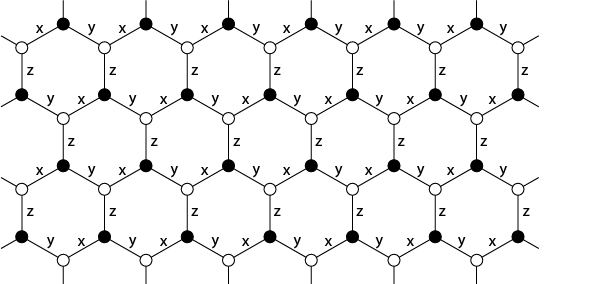
\includegraphics{Kitaev06lattice} &
      \raisebox{1cm}{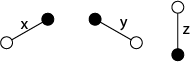
\includegraphics{Kitaev06links}}  \\
(a) & (b)
\end{tabular}}
\caption{Three types of links in the honeycomb lattice.}
\label{fig:Kitaev06_honeycomb}
\end{figure}

\item[2023-10-20 Predrag]
Kitaev reading club with Bader H. Aldossari
\\
<baldossari3@gatech.edu>.
Meetings Zoom 973 4569 4798 `Tigers rule'.

Alexei Kitaev\rf{Kitaev06}\\
{\em Anyons in an exactly solved model and beyond},
\arXiv{cond-mat/0506438}.

So far we have discussed 3 broad topics:
crystalographic \textbf{lattices};
\textbf{group theory};
\textbf{perturbation theory}.

\item[2023-10-21 Predrag] On {\bf lattices}:

Being lazy, everything I do is on the simplest of lattices, the square (or hyper-cubic)
lattice. Currently my favorite exposition is Han's and my
\HREF{https://chaosbook.org/overheads/spatiotemporal/CL18.pdf\#equation.1.1}
{CL18 current draft} of our `deterministic field theory' paper.
I would love to discuss it with you.

But if this exposition is too condensed,
try
\toChaosBook{appendix.X} {Appendix~A24}
{\em Deterministic diffusion}. Things to understand are:

dicretized fields on lattices (I use only bosons; you have a pair of complex fields,
\ie, a `spinor' per lattice site, a 2\dmn\ irrep of internal, lattice site field
su(2) symmetry)


lattice derivatives,
lattice Laplacians,

Periodic lattices, reciprocal lattices, see
\HREF{https://chaosbook.org/overheads/spatiotemporal/CL18.pdf\#section.4}
{CL18 sect.~4. Bravais lattices}.


eigenmodes of translation generators (shift operators)
used to diagonalise (by discrete Fourier
transforms) non-local operators,
such as Laplacians, and invert them;

Green's functions\HREF{https://chaosbook.org/overheads/spatiotemporal/CL18.pdf\#equation.2.61}
{CL18 eq.~(61) }, eq.~(174) and
\HREF{https://chaosbook.org/overheads/spatiotemporal/CL18.pdf\#subsection.8.3}
{CL18 sect.~8.3. \emph{Green’s function of two-dimensional spatiotemporal cat}};

Lattice propagators
\HREF{https://chaosbook.org/overheads/spatiotemporal/CL18.pdf\#equation.3.78}
{CL18 sect.~3.2. \emph{Bravais lattice stability}}.
My favorite derivation of the propagator
\HREF{https://chaosbook.org/FieldTheory/QMlectures/lectQM.pdf\#equation.1.2.21}
{QMlectures eq.~(1.21)} is
\HREF{https://chaosbook.org/FieldTheory/QMlectures/lectQM.pdf\#section.1.1}
{QMlectures sect.~1.1 {\em Wanderings of a drunken snail}}.

\item[2023-10-21 Predrag]
\newcommand{\pcell}{primitive cell}\newcommand{\Pcell}{Primitive cell}

Consider a \textbf{honeycomb lattice} of \reffig{fig:Kitaev06_honeycomb}\,(a).
Under the translation group, its {\pcell} can be taken as a hexagon tile
(lattice plaquette),

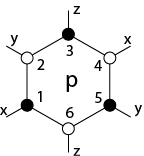
\includegraphics{Kitaev06invariant}
\,,

with dangling links labeled as in \reffig{fig:Kitaev06_honeycomb}\,(b).

If you take as primitive vectors the two unit lattice translations along
$60^o$ and $120^o$ directions, then their sum translate the lattice
by one tile vertically, and their difference generates
one-tile horizontal translation.

That might not be in your taste, as these primitive vectors are
orthogonal to  {\pcell} links.
So view the lattice as consisting of two equivalent simple sublattices,
``even'' and ``odd'' (empty, full circles in the figure).

Shifts along ``$x$-links'', ``$y$-links'', and ``$z$-links'' directions,
\reffig{fig:Kitaev06_honeycomb}\,(b), independent translations
along $x$ and $y$ directions, $z$ translation given by the sum
-$x$-link - $y$-translation, translate the 2 triangular sublattices
into each other. The lattice is invariant under pairs of
successive different shifts. For example, successive shifts, first along
$x$-links'', than along ``$y$-links translate the lattice by one lattice unit in the $z$ direction

The point group of either sublattice is $\Dn{3}$, 3 rotations, and 3
reflections. A sensible theory should also be invariant under
interchanging the two sublattices. Under all these discrete symmetries,
the honeycomb is built from Kitaev's `unit cell' that contains one vertex
of each kind.

The Hamiltonian
\begin{equation} \label{Kitaev06:Hamiltonian}
H\,=\,
-J_{x} \sum_{\text{$x$-links}} \sigma_{j}^{x}\sigma_{k}^{x}
-J_{y} \sum_{\text{$y$-links}} \sigma_{j}^{y}\sigma_{k}^{y}
-J_{z} \sum_{\text{$z$-links}} \sigma_{j}^{z}\sigma_{k}^{z},
\end{equation}
where $J_{x}$, $J_{y}$, $J_{z}$ are parameters, is a sparse,
almost diagonal (almost = the nearest neighbors) operator (an infinite
matrix acting on the infinite honeycomb lattice) of a block diagonal
form: it acts on lattice site 2-component 1/2-spin field with a 2\dmn\
local matrix (Pauli matrices, the identity). Were $J_{x}=J_{y}=J_{z}$,
one could write it as a Laplacian (see
\HREF{https://chaosbook.org/overheads/spatiotemporal/CL18.pdf\#equation.2.49}
{CL18 eq.~(2.49)}), with zero Klein-Gordon mass `potential'.
Bader, can you do this exercise? I do not remember doing it.

The individual operators in the Hamiltonian:
\begin{equation} \label{terms}
K_{jk}= \left\{
\begin{array}{l@{\quad}l}
\sigma_{j}^{x}\sigma_{k}^{x}, & \text{if $(j,k)$ is an $x$-link;} \\
\sigma_{j}^{x}\sigma_{k}^{y}, & \text{if $(j,k)$ is an $y$-link;} \\
\sigma_{j}^{x}\sigma_{k}^{z}, & \text{if $(j,k)$ is an $z$-link.}
\end{array}
\right.
\end{equation}
Remarkably, \emph{all} operators $K_{jk}$
commute with lattice plaquette (i.e., hexagon) operators
$W_{p}$:
\begin{equation} \label{Kitaev06:invariant}
\begin{array}{c} 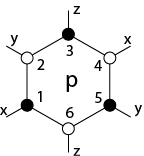
\includegraphics{Kitaev06invariant} \end{array} %\qquad\quad
W_{p}=\sigma_{1}^{x}\sigma_{2}^{y}\sigma_{3}^{z}
\sigma_{4}^{x}\sigma_{5}^{y}\sigma_{6}^{z}
=K_{12}K_{23}K_{34}K_{45}K_{56}K_{61}.
\end{equation}
It's probably not remarkable. As explained above, any non-repeating pair
of shifts along $x$-, $y$-, $z$-links is a unit lattice translation. The
three consecutive such in the chain \refeq{Kitaev06:invariant} add up to
a zero translation, so anything will commmute with it, including
operators $K_{jk}$, and different operators $W_{p'}$.

\item[2023-10-17 Predrag] On \textbf{group theory}:

Kitaev06 \HREF{https://arxiv.org/pdf/cond-mat/0506438.pdf\#equation.3.20}
{eq.~(20)} follows from the definition of a tensor,
\HREF{https://birdtracks.eu/version9.0/GroupTheory.pdf\#equation.3.2.26}
{birdtracks.eu eq.~(3.26)}:
a finite `rotation' of an
$n$-legged tensor rotates each leg (a `leg' is a free, not contracted index).

$e^{-iT\cdot\theta} M e^{iT\cdot\theta}$
is just how a Hermitian matrix $M$ (2-index tensor, one index up, one
down) transforms, Heisenberg version of the Schr{\"o}dinger equation
being a special case. As time evolution is a 1\dmn\,
abelian group, you don't even see an adjoint index.
Basically, Heisenberg is a statement of finite time
evolution,  Schr{\"o}dinger is the infinitesimal time step $=$
differential equation version.

I find the infinitesimal statement of tensor invariance,
\HREF{https://birdtracks.eu/version9.0/GroupTheory.pdf\#equation.4.4.36}
{birdtracks.eu eq.~(4.36)} and
{(4.33)},
easier to grasp.

If $M$ is built from $N$ generators in the $N$\dmn\ adjoint representations
2 indices shared with $M$, but the 3rd index in the adjoint rep (like 3
Pauli matrices, the generators of su(2)),  then various commutators give
structure constants $c_{ijk}$. They are generators of adjoint
representation rotations, hence the rotation matrix on the right hand
side of Kitaev06 {eq.~(20)}.

Examples:\\
\HREF{https://birdtracks.eu/course3/notes.pdf\#equation.10.5.10}
{eq.~(10.10)},
\HREF{https://birdtracks.eu/course3/notes.pdf\#equation.11.2.4}
{eq.~(11.4)} and thereabouts,
\HREF{https://birdtracks.eu/course3/notes.pdf\#equation.12.3.7}
{eq.~(12.7)}  and thereabouts,
but much of it is special to so(4) being a semisimple su(2)$\times$su(2),
misleading about the general case. My notes are \emph{not} a textbook
on group theory, only pointers to the literature. To learn it my way, you
need to go through videos listed at the beginning of each chapter, read
the literature if suggested.

\item[2023-10-21 Predrag]

I do spin representations in
\HREF{https://birdtracks.eu/version9.0/GroupTheory.pdf\#section.11.1}
{birdtracks.eu sect.~11.1},
but that is probably too tough (for anyone:).
If you can get through spinsters,
\HREF{https://birdtracks.eu/version9.0/GroupTheory.pdf\#section.14.1}
{birdtracks.eu sect.~14.1}, my hat off to you:)
My birdtracks are good if you have to do real calculations (like
perturbative corrections). On a superficial level, standard literature is
good enough.

\item[2023-10-21 Predrag] On {\bf perturbation expansions}:

Currently my favorite bosonic field theory is scalar $\phi^4$ any
dimension, in practice in 1 and 2 dimensions.

We work at Klein-Gordon mass-square values where perturbation theory
in powers of the coupling strength of the nonlinear potential makes
no sense.  Our
potential term $\phi^4$ dominates over the `kinetic', Laplacian term.
This is known as the
anti-integrable limit
\HREF{https://chaosbook.org/overheads/spatiotemporal/CL18.pdf\#equation.3.73}
{CL18 eq.~(73)}
in the current draft of our `deterministic field theory' paper.

Kitaev06 Hamiltonian \refeq{Kitaev06:Hamiltonian} only has a `kinetic',
Laplacian term. It has no on-site potential
or spinor mass - it's a massless theory.

So Kitaev06, in
\HREF{https://arxiv.org/pdf/cond-mat/0506438.pdf\#subsection.5.10}
{5.1 {\em Perturbation theory study} }, breaks
the honeycomb \Dn{6} symmetry by singling out the vertical
$z$-links in
\reffig{fig:Kitaev06_honeycomb}\,(b),
and combines the $x$- and $y$-links into generators of horizontal
translations, his `potential' V, resulting in a $\Dn{2}\times\Dn{2}$
`non-relativisitc'
rectangular latice; lattice `constants'
or `coupling strengths' or `speed of light'
are different in the horizontal and vertical directions:

Kitaev06 Hamiltonian is $H=H_{0}+V$, where $H_{0}$ is the main part and $V$ is the
perturbation:
\[
H_{0} = -J_{z} \sum_{\text{$z$-links}} \sigma_{j}^{z}\sigma_{k}^{z},
\qquad\quad
V = -J_{x} \sum_{\text{$x$-links}} \sigma_{j}^{x}\sigma_{k}^{x}
-J_{y} \sum_{\text{$y$-links}} \sigma_{j}^{y}\sigma_{k}^{y}
\]
The important thing is that $H_0$ generates vertical translations, $V$
horizontal translation, so they commute. The propagator can be expanded
as a geometrical series in terms of the small parameter $J_{x}=J_{y}$,
\beq
\frac{1}{H_{0} + V} =
\frac{1}{H_{0}} \sum_{n=0}^{\infty}\left({H_{0}^{-1}{V}}\right)^n
\,,
\ee{Kitaev06:PertSeries}
and computes the first four terms. It's a calculation, as there are
various powers of Pauli matrices in various terms.  Odd terms vanish,
because you need even powers of $V$ to get to lattice translations.

As $\Dn{2}\times\Dn{2}$ includes symmetries under reflections across $x$
and $z$ axes, I believe that one could have written the theory in a Dirac
propagator form, linear in 'momentum', from the start, but working that
out might merit a stand-alone publication.

Kitaev06 first sets to the anti-integrable limit $J_{z}\to\infty$,
or $J_{x}=J_{y}=0$.
In that case this is a 1\dmn\ latice,
with  $\Dn{2}$ symmetry. Its ground state is highly
degenerate: each two spins connected by a $z$-link are aligned
( spinup spinup  or  spindown spindown), but their common direction is
not fixed.
% We regard each such pair as an effective spin.
% The transition from physical spins to effective spins is shown in
% Fig.~\ref{fig_perturb}a,b.
The ground state energy is $E_{0}=-NJ_{z}$,
where $N$ is the number of unit cells, i.e., half the number of spins.

I stop here - do not know whether this is helpful to Bader,
until he finds it helpful.





Come back when you get to the next hurdle.

\item[2023-10-xx Bader]














\item[2018-06-16 Predrag]
Remember to send Henry Ki{\ss}ler a hard copy of my ``Field Theory''
book\rf{FieldThe}.


\end{description}


%\newpage %%%%%%%%%%%%%%%%%%%%%%%%%%%%%%%%%%%%%%%%%%%%%%%%
\printbibliography[heading=subbibintoc,title={References}]
